
\فصل{نتایج جدید}

در این فصل نتایج جدید به‌دست‌آمده در پایان‌نامه توضیح داده می‌شود.
در صورت نیاز می‌توان نتایج جدید را در قالب چند فصل ارائه نمود.
همچنین در صورت وجود پیاده‌سازی، بهتر است نتایج پیاده‌سازی را 
در فصل مستقلی پس از این فصل قرار داد.

\قسمت{الگوریتم تقسیم و حل}

در این بخش الگوریتمی را ارائه خواهیم داد که مسئله‌ی تنظیم دقیق آستانه‌ها را برای یک شبکه‌ی پرسپترون سه‌لایه که شمای آن در شکل \رجوع{شکل:schematicNN} ارائه شده بود حل کند. تعریف دقیقی در مسئله در ادامه ارائه شده است.


\شروع{مسئله}[تنظیم دقیق آستانه‌ها]
برای یک شبکه‌ی پرسپترون سه‌لایه با ابعاد
$d \times h \times 1$
نورون با وزن‌های داده‌شده‌ی
$w_1, \dots, w_d \in \mathbb{R}^{h}$
و مجموعه‌ی $n$ داده‌ی برچسب‌دار
$(x^{(j)}, y^{(j)}) \in \mathbb{R}^{d} \times \{0, 1\}$
که خروجی شبکه روی هر داده‌ی ورودی توسط تابع زیر محاسبه می‌شود:
\begin{equation} \label{eq:network}
	F(x) = \sigma\left( \tau + \sum_{i=1}^h v_i \sigma(w_i^T x + b_i)\right)
\end{equation}
مطلوب است یافتن مقادیر بهینه‌ی آستانه، $b=(b_1, \dots, b_d)$ و نیز $\tau$، چنان‌که تعداد داده‌های ورودی که خروجی شبکه برای آن‌ها برابر با برچسب‌شان است بیشینه شود:

\begin{equation*} \label{eq:argmax}
	b_{\OPT}, \tau_{\OPT} = \argmax_{b, \tau} \sum_{j=1}^N I(F(x^{(j)}) = y^{(j)})
\end{equation*}

\پایان{مسئله}

برای این مسئله، یک الگوریتم تقسیم و حل ارائه خواهیم داد که بر پایه‌ی الگوریتم چان \مرجع{chan2013easy} برای حل مسئله‌ی عمق است. فرض کنید زیرمجموعه‌ی $\mathcal{S}$ از نورون‌های لایه‌ی نهان داده شده که مقدار آستانه‌ی آن‌ها قابل تنظیم است. همچنین فرض کنید که برای یک ورودی دلخواه
$x^{(j)}$
مایلیم مقادیر آستانه را به‌گونه‌ای تنظیم کنیم که خروجی شبکه با برچسب خروجی آن برابر باشد. اکنون
$2^d$
زیرمجموعه از نورون‌های لایه‌ی نهان را درنظر می‌گیریم که هرکدام حالتی را مشخص می‌کنند از فعال‌بودن تعدادی از نورون‌ها و غیرفعال‌بودن بقیه. فعال یا غیرفعال بودن نورون $i$-ام از لایه‌ی نهان، یک محدودیت خطی روی مقدار آستانه‌ی آن را اعمال می‌کند؛ اگر آن نورون فعال باشد، باید شرط زیر برقرار باشد:
$$w_i^T x^{(j)} + b_i \ge 0 \Rightarrow b_i \ge -w_i^T x^{(j)}$$
و اگر غیرفعال باشد، شرط معکوس زیر باید برقرار باشد:
$$w_i^T x^{(j)} + b_i < 0 \Rightarrow b_i < -w_i^T x^{(j)}$$
اگر شرط‌هایی که به ازای هر زیرمجموعه از نورون‌های فعال روی بردار $b$ اعمال می‌شود را لحاظ کنیم،
$2^d$
می‌توانیم آن‌ها را به صورت
$2^d$
جعبه در فضای $d$-بعدی نشان دهیم که مجزا هستند و این فضا را افراز می‌کنند.

حال مسئله را بسته به آنکه آستانه‌ی لایه‌ی آخر ($\tau$) قابل تنظیم یا ثابت باشد دو حالت می‌کنیم. اگر حالت ثابت را در نظر بگیریم، برای هر یک از $2^d$ حالت از فعال یا غیرفعال‌بودن نورون‌های لایه‌ی نهان می‌توانیم مشخص کنیم که خروجی شبکه با برچسب
$y^{(j)}$
برابر شده است یا نه. برای هر ورودی، اگر بردار $b$ درون یکی از جعبه‌های متناظر با چنین حالتی باشد، شبکه یک امتیاز در رابطه‌ی \رجوع{eq:loss} خواهد گرفت. پس اگر برای $n$ داده‌ی ورودی
$2^d \times n$
جعبه بسازیم و الگوریتم چان را بری حل مسئله‌ی عمق در این فضا به کار بگیریم، مقادیری برای آستانه‌های $b$ را خواهیم یافت که بیشترین امتیاز را روی مجموعه‌ی دادگان ورودی خواهند گرفت. یادآوری می‌شود که جعبه‌های مرتبط با هر داده‌ی ورودی مجزا هستند، پس هر تقاطع نقطه‌ی $b$ با یک جعبه، یک امتیاز برای داده‌ای متفاوت را برای شبکه نشان می‌دهد.

از سوی دیگر اگر $\tau$ نیز قابل تنظیم باشد، به ازای هرکدام از حالت‌های فعال یا غیرفعال بودن نورون‌های لایه‌ی نهان، مشابه با حالت قبل محدودیت‌هایی روی مقادیر $b_1$ تا $b_d$ خواهیم داشت و این بار افزون بر آن، اگر خروجی مدنظر برای نورون‌های لایه‌ی نهان را با $F_1$ تا $F_d$ نشان دهیم، یک محدودیت روی مقدار $\tau$ خواهیم داشت تا بسته به آنکه برچسب خروجی یک یا صفر باشد، خروجی شبکه (که از رابطه‌ی \رجوع{eq:network} به‌دست می‌آید) با آن برچسب برابر شود:

\begin{equation*}
	\tau \mathop{\gtreqless}_{y^{(j)}=0}^{y^{(j)}=1} -\sum_{i=1}^h v_i F_i
\end{equation*}

پس در این حالت هم می‌توان بخش مطلوب از فضای جستجو برای مقادیر آستانه‌ها را که برای یک داده‌ی ورودی منجر به کسب امتیاز برای شبکه می‌شود توسط $2^d$ جعبه در فضای $\mathbb{R}^{d+1}$ نشان داد، و مجدداً کافیست مسئله‌ی عمق را در فضای جستجوی مقادیر آستانه‌ها برای
$2^d \times n$
جعبه حل کنیم.

... خود الگوریتم و تحلیلش باید سپس نوشته شود ...


%%%%%%%%%%%%%%%%%%%%%%%%%%%%%%%%%%%%%%%%%%%%%%%
%%%%%%%%%%%%%%%%%%%%%%%%%%%%%%%%%%%%%%%%%%%%%%%
%%%%%%%%%%%%%%%%%%%%%%%%%%%%%%%%%%%%%%%%%%%%%%%


\قسمت{کاهش پارامتری}

\شروع{لم}
مسئله‌ی یافتن یک خوشه با $d$ رأس در گرافی با $n$ رأس و $m$ یال قابل کاهش است به مسئله‌ی عمق در فضای $d$-بعدی با
$4\binom{d}{2}(n^2 - 2m) + 1$
جعبه.
\پایان{لم}

\شروع{اثبات}
ابتدا یک جعبه‌ی اولیه به شکل
$<(0,0,...,0), (n, ..., n)>$
در نظر می‌گیریم. همچنین رئوس گراف را از $0$ تا $n-1$ نام‌گذاری می‌کنیم. سپس اگر مجموعه‌ی یال‌های گراف را $E$ بنامیم، برای هر زوج‌مرتب $(u,v)$ که $\{u,v\} \notin E$ و برای هر $i, j \in  \{0, \dots n-1\}$ که $i<j$ باشد، چهار جعبه به صورت زیر تعریف می‌کنیم:

\begin{align*}
	B_{i,j,u,v,00} &= <(\underset{i-1}{\underbrace{-\infty, ..., -\infty}}, u, -\infty, ..., -\infty), (\underset{j-1}{\underbrace{+\infty, ..., +\infty}}, v, +\infty, ..., +\infty)>\\
	B_{i,j,u,v,11} &= <(\underset{j-1}{\underbrace{-\infty, ..., -\infty}}, v+1, -\infty, ..., -\infty), (\underset{i-1}{\underbrace{+\infty, ..., +\infty}}, u+1, +\infty, ..., +\infty)>\\
	B_{i,j,u,v,01} &= <(-\infty, ..., -\infty), (\underset{i-1}{\underbrace{+\infty, ..., +\infty}}, u, \underset{j-i-1}{\underbrace{+\infty, ..., +\infty}}, v+1, +\infty, ..., +\infty)>\\
	B_{i,j,u,v,10} &= <(\underset{i-1}{\underbrace{-\infty, ..., -\infty}}, u+1, \underset{j-i-1}{\underbrace{-\infty, ..., -\infty}}, v, -\infty, ..., -\infty),(+\infty, ..., +\infty)>\\
\end{align*}

به سادگی می‌توان مشاهده کرد که این چهار جعبه مجزا هستند و در نتیجه هر نقطه‌ی دلخواه $p$ در فضای $d$-بعدی حداکثر در یکی از این چهار جعبه قرار دارد. در واقع اگر
$u \le p_i < u + 1$ و $v  \le p_j < v+1$
باشد، نقطه‌ی $p$ در یکی از این چهار جعبه قرار دارد؛ و در غیر این صورت، خارج از این چهار جعبه است.

حال می‌توانیم این جعبه‌ها را به عنوان ورودی مسئله‌ی عمق در نظر بگیریم و بررسی کنیم که آیا جواب آن برابر با
$\binom{d}{2}(n^2 - 2m) + 1$
است یا خیر. از آنجا که چهار جعبه‌ی متناظر با $i,j,u,v$ اشتراکی ندارند، رسیدن به جواب فوق تنها در حالتی رخ می‌دهد که نقطه‌ی $p$ وجود داشته باشد که هم در جعبه‌ی اولیه باشد (به بیان دیگر تمام اندیس‌های $i$ داشته باشیم 
$0 \le p_i < n$
) و هم برای تمام اندیس‌های $i,j,u,v$، نقطه‌ی $p$ در حداقل یکی از چهار جعبه‌ی متناظر باشد. وجود چنین نقطه‌ای به این معناست که هیچ دو اندیس $i, j$ و هیچ $\{u,v\} \notin E$ وچود نداشته باشد که
$u \le p_i < u + 1$ و $v  \le p_j < v+1$
باشد. گزاره‌ی فوق به این معناست که برای هر $i, j$ که
$i \neq j$
داشته باشیم
$\{\lfloor p_i \rfloor, \lfloor p_j \rfloor\} \in E$.
پس هر دو مختصات از نقطه‌ی $p$ توسط یک یال به هم متصل‌اند، و وجود این نقطه به معنای وجود یک خوشه‌ی $d$ رأسی در گراف است.

\پایان{اثبات}

اکنون می‌توان نتیجه گرفت که مسئله‌ی عمق در زمان $O(f(d) n^{o(d)})$ قابل حل نیست، زیرا مسئله‌ی پارامتری خوشه بنا به فرض ETH در زمان $O(f(d) n^{o(d)})$ قابل حل نیست.

حال که یک کاهش از مسئله‌ی خوشه به مسئله‌ی عمق داریم، به سراغ ارائه‌ی کاهشی از مسئله‌ی عمق به مسئله‌ی تنظیم دقیق آستانه (برای شبکه‌ی پرسپترون سه‌لایه تصویرشده در شکل~\رجوع{شکل:schematicNN}) می‌رویم. با این حال، بررسی ما نشان داده که بسته به اینکه مقدار آستانه برای نورون لایه‌ی آخر (که آن را با $\tau$ نشان می‌دهیم) ثابت یا قابل تنظیم باشد، طبیعت مسئله متفاوت خواهد بود. به همین دلیل، در ادامه و در دو لم مجزا به هر کدام می‌پردازیم.

\شروع{لم}
مسئله‌ی عمق با $k$ جعبه در فضای $d$-بعدی قابل کاهش است به مسئله‌ی تنظیم دقیق آستانه‌ها برای یک شبکه‌ی پرسپترون سه‌لایه با تابع فعال‌ساز پله و یک لایه‌ی نهان با $d$ نورون، روی یک مجموعه‌ی دادگان ورودی به اندازه‌ی $k \times 2^d$، در حالی که مقدار آستانه‌ی لایه‌ی آخر \textbf{ثابت} باشد.
\پایان{لم}

\شروع{اثبات}
یک ورودی برای مسئله‌ی عمق (شامل $k$ جعبه در فضای $d$-بعدی) را در نظر می‌گیریم. در ابتدا، یک عدد مثبت $M$ به اندازه‌ی کافی بزرگ را پیدا می‌کنیم که مختصات گوشه‌های تمام جعبه‌ها بین $M$ و $-M$ باشد. حال اگر جعبه‌هایی بی‌کران داشتیم (که طبق تعریف مسئله‌ی عمق مجاز است)، کران‌های نامحدود $-\infty$ را با $-M$ و کران‌های $+\infty$ را با $+M$ جایگزین می‌کنیم. پاسخ مسئله‌ی عمق با این جایگزینی تغییری نمی‌کند.


\شروع{شکل}[ht]
\centering
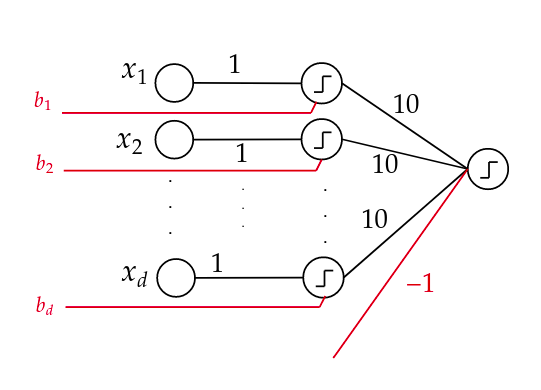
\includegraphics[scale=0.5]{figs/reductionKnownThreshold.png}
\شرح{یک شبکه‌ی پرسپترون سه‌لایه که برای کاهش مسئله‌ی عمق به مسئله‌ی تنظیم دقیق آستانه استفاده می‌کنیم. لایه‌ی آخر در این شبکه نقش یک «یای منطقی» را ایفا می‌کند به‌گونه‌ای که نورون خروجی شبکه فعال خواهد شد اگر و تنها اگر حداقل یکی از نورون‌های لایه‌ی نهان فعال شوند.}
\برچسب{شکل:reductionKnownThreshold}
\پایان{شکل}

سپس از شبکه‌ی عصبی که در شکل~\رجوع{شکل:reductionKnownThreshold} به تصویر کشیده شده استفاده می‌کنیم و مجموعه‌ی دادگان برای تنظیم دقیق را در ادامه تعریف می‌کنیم. برای هر زیرمجموعه مانند $S$ از
$\{0, \dots d-1\}$
و هر جعبه‌ی
${B= <(l_1, l_2, ..., l_d), (r_1, ..., r_d)>}$
یک زوج $(x^{(S, B)}, y^{(S, B)})$ با مقادیر زیر به مجموعه‌ی دادگان ورودی شبکه‌ی عصبی اضافه می‌کنیم:

\begin{equation}
	x^{(S, B)} = \begin{pmatrix} x^{(S, B)}_1 & x^{(S, B)}_2 & \hdots & x^{(S, B)}_d\end{pmatrix}, x^{(S, B)}_i = \begin{cases}
	r_i & i \in S\\
	l_i & i \notin S
\end{cases} \label{eq:xs}
\end{equation}
\begin{equation}
 	y^{(S, B)} = \begin{cases}
	0 & |S| \overset{2}{\equiv} d\\
	1 &  |S| \overset{2}{\not\equiv} d
\end{cases} \label{eq:ys}
\end{equation}

به ازای هر جعبه، مجموعه‌ی دادگان فوق حاوی $2^d$ به شکل زوج مرتب است که اعضای اول آن‌ها متناظر با $2^d$ گوشه‌ی آن جعبه هستند. همچنین اعضای دوم، به شکل برچسب‌هایی دودودیی هستند که زوجیت\پاورقی{parity} گوشه‌ها را نشان می‌دهند. زوجیت یک گوشه از جعبه‌ی $B$، زوجیت تعداد محورهایی است که آن گوشه در آن محور با کران بالای جعبه ($r_i$) مقداردهی شده است. به عنوان مثال زوجیت گوشه‌ی $(l_1, l_2, ..., l_d)$ برابر با صفر است.

اکنون خود را محدود به مجموعه‌ی دادگان مرتبط با فقط یک جعبه مثل $B_1$ می‌کنیم، که حاوی $2^d$ داده است. ادعا می‌کنیم که اگر مقدار انتخابی برای مقادیر آستانه‌ی
$b = (b_1, \dots, b_d)$
معادل با نقطه‌ای خارج جعبه‌ی $B_1$ باشد، امتیاز شبکه‌ی عصبی یا به عبارت دیگر تعدادی از داده‌هایی که خروجی شبکه با برچسب آن‌ها یکسان است برابر با
$2^{d-1}$
می‌شود، و اگر $b$ متناظر با نقطه‌ای داخل جعبه باشد، این امتیاز
$2^{d-1}+1$
می‌شود. اگر این ادعا ثابت شود، تنظیم دقیق آستانه‌های شبکه‌ی شکل~\رجوع{شکل:reductionKnownThreshold} (که همان بهینه‌کردن مقدار بردار آستانه‌های $b$ است به گونه‌ای که امتیاز شبکه روی مجموعه‌ی دادگان ساخته‌شده از روی جعبه‌ها بیشینه شود) معادل با یافتن نقطه‌ای درون بیشترین تعداد جعبه‌ها خواهد بود.

یک انتخاب برای مقادیر آستانه به صورت
$b = (b_1, \dots, b_d)$
را برای شبکه‌ی شکل~\رجوع{شکل:reductionKnownThreshold} در نظر بگیرید. باتوجه به ساختار این شبکه، نورون $i$-ام لایه‌ی نهان به شرطی فعال می‌شود که
$x_i \leq b_i$
باشد. همچنین خروجی شبکه در صورتی که حداقل یکی از نورون‌های لایه‌ی نهان فعال شود برابر با یک، و در غیر این صورت برابر با صفر است.

برای سادگی، یک انتخاب برای بردار $b$ را با رشته‌ای از نمادهای '$\sqcup$'، '$+$' و '$-$' نشان می‌دهیم. اگر $l_i \leq b_i < r_i$ باشد نماد $i$-ام در رشته‌ی متناظرش را '$\sqcup$' قرار می‌دهیم، اگر $b_i \geq r_i$ باشد آن را با '$+$' نشان می‌دهیم، و نهایتاً اگر $b_i < l_i$ باشد آن را با '$-$' نشان می‌دهیم. در ادامه نشان خواهیم داد که برای هر نقطه‌ی $b$ که رشته‌ی متناظرش هر چیزی به‌جز "$\sqcup\sqcup ... \sqcup$" باشد امتیاز شبکه‌ی عصبی برابر با $2^{d-1}$ است و برای این رشته‌ی خاص که نمایان‌گر نقطه‌ی داخل جعبه‌ی $B_0$ است امتیاز شبکه برابر با
$2^{d-1}+1$
است.

ابتدا نقاطی را در نظر بگیرید که رشته‌ی متناظرشان حداقل یک نماد '$+$' داشته باشد. در این حالت می‌دانیم که حداقل یک نورون فعال خواهد شد، پس شبکه‌ی عصبی فقط برای داده‌هایی با
$y^{(S, B_1)}=1$
امتیاز خواهد گرفت. تعداد چنین داده‌هایی برابر با $2^{d-1}$ است، که متناظر با تعداد زیرمجموعه‌هایی مانند $S$ است که $|S|$ زوجیتی متفاوت از $d$ داشته باشد. به طور مشابه نشان داده می‌شود که اگر رشته‌ی متناظر با بردار $b$ تنها شامل نماد '$-$' باشد، هیچ نورون لایه‌ی نهان فعال نخواهد شد و شبکه فقط امتیاز داده‌هایی با برچسب
$y^{(S, B_1)}=0$
را خواهد گرفت که آن‌ها نیز $2^{d-1}$ هستند.

اکنون نقاطی را در نظر بگیرید که رشته‌ی متناظرشان به تعداد $t$ واحد نماد '$\sqcup$' و به تعداد $d-t$ واحد نماد '$-$' دارد. برای داده‌ای با برچسب صفر، شبکه‌ی عصبی تنها در صورتی امتیازش را می‌گیرد که در اندیس‌هایی متناظر با نماد '$\sqcup$'، ورودی $x_i^{(S,B_1)}$ برابر با $l_i$ باشد؛ زیرا در غیر این صورت نورون $i$-ام فعال خواهد شد و خروجی شبکه‌ی عصبی صفر نخواهد بود. برای اندیس‌های دیگر فارغ از اینکه $x_i^{(S,B_1)}$ برابر با $l_i$ یا $r_i$ باشد، نورون $i$-ام فعال نخواهد شد. با این حال زیرمجموعه‌ی $S$ از اندیس‌ها باید به‌گونه‌ای انتخاب شود که
$|S| \overset{2}{\equiv} d$
تا برچسب خروجی صفر باشد. پس برای
$2^{d-t-1}$
داده با برچسب صفر، شبکه‌ی عصبی امتیازشان را می‌گیرد. برای داده‌های با برچسب یک، کافیست حداقل برای یک اندیس $i$ از $t$ اندیسی که متناظر با نماد '$\sqcup$' هستند داشته باشیم $x_i=l_i$؛ تا نورون $i$-ام و در نتیجه خروجی شبکه‌ی عصبی فعال شود. برای اندیس‌های متناظر با نماد '$-$' فارغ از اینکه ورودی چه باشد، نورون متناظرشان فعال نخواهد شد. پس $2^t-1$ انتهاب برای اندیس‌های دسته‌ی اول و سپس $2^{d-t-1}$ انتخاب برای اندیس‌های باقی‌مانده داریم تا به داده‌هایی با برچسب یک برسیم که خروجی شبکه‌ی عصبی هم فعال باشد. در مجموع، تعداد داده‌هایی که شبکه‌ی عصبی امتیازشان را در این حالت می‌گیرد برابر است با

$$2^{d-t-1} + (2^t-1) \times 2^{d-t-1} = 2^{d-1}.$$

اکنون به بررسی تنها حالت باقی‌مانده می‌پردازیم که انتخاب برای $b$ متناظر با رشته‌ای تنها شامل نمادهای '$\sqcup$' باشد (که به معادل نقطه‌ای درون جعبه‌ی $B_1$ است). برای داده‌های با یرچسب صفر، هیچ‌کدام از نورون‌های لایه‌ی نهان نباید فعال شوند؛ پس برای تمام اندیس‌ها باید $x_i=r_i$ باشد یعنی
${ S=\{1, \dots, d\} }$ 
باشد. از آنجا که در این حالت
$|S| \overset{2}{\equiv} d$
است، پس مطابق رابطه‌ی
\رجوع{eq:ys}
خروجی شبکه‌ی عصبی با برچسب داده مطابقت خواهد داشت. برای داده‌های با برچسب یک، کافیست حداقل یک $x_i$ برابر با $l_i$ باشد تا نورون $i$-ام و در نتیجه خروجی شبکه فعال شود، و نیز
$|S| \overset{2}{\equiv} (d-1)$
باشد تا شرط برچسب یک تضمین شود. برای برقراری شرط هم‌نهشتی $2^{d-1}$ انتخاب برای زیرمجموعه‌ی $S$ داریم که به سادگی مشاهده می‌شود در تمام آن‌ها حداقل برای یک اندیس $i$، شرط $x_i=r_i$ برقرار است. پس در مجموع در این حالت امتیاز شبکه برابر است با
$2^{d-1}+1$.

در نتیجه می‌توانیم به ازای $k$ جعبه‌ی ورودی، یک مجموعه‌ی دادگان با اندازه‌ی
$2^d k$
بسازیم و با بیشینه‌کردن امتیاز شبکه‌ی
شکل \رجوع{شکل:reductionKnownThreshold}
چنان‌که در رابطه‌ی \رجوع{eq:loss} آمده است، به امتیاز
$2^{d-1} \times k + T$
برسیم که $T$ تعداد جعبه‌هایی است که بردار بهینه‌ی $b$ یا همان مقادیر آستانه‌ی نورون‌ها درون آن جعبه‌ها قرار می‌گیرد. پس با تفریق مقدار
$2^{d-1} \times k$
از پاسخ مسئله‌ی تنظیم دقیق آستانه‌ها، می‌توانیم پاسخ مسئله‌ی عمق را بیابیم. پس درستی کاهش نشان داده شد.
\پایان{اثبات}

\شروع{لم}
مسئله‌ی عمق با $k$ جعبه در فضای $d$-بعدی قابل کاهش است به مسئله‌ی تنظیم دقیق آستانه‌ها برای یک شبکه‌ی پرسپترون سه‌لایه با تابع فعال‌ساز پله و یک لایه‌ی نهان با $d$ نورون، روی یک مجموعه‌ی دادگان ورودی به اندازه‌ی $k \times 2^d$، در حالی که مقدار آستانه‌ی لایه‌ی آخر \textbf{قابل تنظیم} باشد.
\پایان{لم}

\شروع{اثبات}

\شروع{شکل}[ht]
\centering
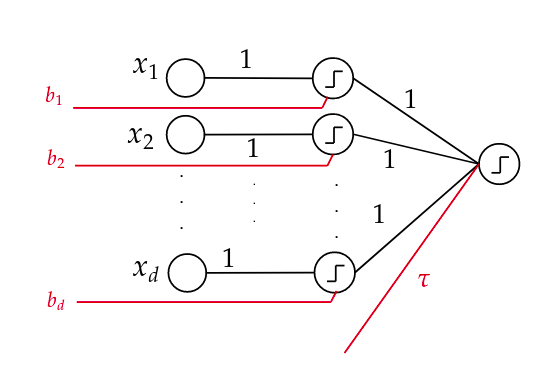
\includegraphics[scale=0.5]{figs/reductionUnknownThreshold.png}
\شرح{یک شبکه‌ی پرسپترون سه‌لایه که برای کاهش مسئله‌ی عمق به مسئله‌ی تنظیم دقیق آستانه در حالتی که آستانه‌ی نورون خروجی قابل تنظیم باشد.}
\برچسب{شکل:reductionUnknownThreshold}
\پایان{شکل}

برای این بخش هم مجموعه‌ی دادگان ورودی را مشابه لم قبل و به ازای $2^d$ گوشه‌ی هر جعبه می‌سازیم، و مشابه لم قبل جعبه‌های بی‌کران را محدود می‌کنیم. اما این بار از یک شبکه با وزن‌های متفاوت استفاده می‌کنیم که در شکل \رجوع{شکل:reductionUnknownThreshold} آمده است.

برای آنکه یک انتخاب برای $b$ روی یک ورودی $x$ با برچسب $y$ امتیاز بگیرد ابتدا باید تعداد نورون‌های فعال‌شده در لایه‌ی نهان را بشماریم؛ یعنی تعداد اندیس‌هایی که
$b_i - x_i \ge 0$
باشد. اگر این تعداد را $t$ بنامیم، آستانه‌ی نورون لایه‌ی خروجی ($\tau$) محدود به $t$ خواهد بود: بسته به اینکه برجسب خروجی برابر با صفر یا یک باشد، مقدار $\tau$ باید بزرگتر از یا کوچکترمساوی با $t$ باشد.

اکنون نشان می‌دهیم مستقل از اینکه چه مقداری برای $\tau$ انتخاب کنیم، اگر بردار
${b = (b_1, \dots, b_d)}$
خارج از جعبه‌ی $B$ باشد، شبکه همیشه امتیاز $2^{d-1}$ را روی مجموعه‌ی دادگان متناظر با گوشه‌های جعبه‌ی $B$ خواهد گرفت. زیرا اگر $b \not\in B$ باشد پس مجموعه‌ای از اندیس‌های $i$ وجود دارند که $b_i$ در بازه‌ی
$[l_i, r_i)$
نباشد. اولین اندیس با این ویژگی را درنظر بگیرید و آن را $j$ بنامید، و ابتدا فرض کنید $b_i < l_i$ باشد.
هر داده‌ی ورودی شبکه که متناظر با زیرمجموعه‌ی
$S \subseteq \{1, \dots, d\}$
است می‌تواند با داده‌ی متناظر با زیرمجموعه‌ی $S'$ جفت شود، که با حذف یا اضافه‌کردن اندیس $j$ به مجموعه‌ی $S$ حاصل می‌شود:
$S' = S \oplus \{j\}$.
از آنجا که $b_j$ پیش از بازه‌ی
$[l_j, r_j)$
در نظر گرفته شد، نورون $j$-ام مستقل از آنکه
$x_j = l_j$
یا
$x_j = r_j$
باشد، همیشه غیرفعال خواهد بود. اما داده‌های متناظر با یکی از دو مجموعه‌ی $S$ و $S'$ یکی دارای برچسب صفر و دیگری دارای برچسب یک است زیرا اندازه‌های این دو مجموعه زوجیتی متفاوت دارند. ابن بدان معناست که هرطور $\tau$ و باقی مقادیر آستانه مقداردهی شوند، شبکه از هر جفت داده دقیقاً یک امتیاز خواهد گرفت. استدلالی مشابه را می‌توان برای حالتی آورد که $b_j \ge r_i$ باشد. پس برای هر جعبه‌ی $B$ که $b \not\in B$ باشد، شبکه امتیاز نیمی از دادگان مرتبط با آن، یعنی امتیاز $2^{d-1}$ داده را خواهد گرفت.

از طرف دیگر، حالتی را در نظر بگیرید که $b$ درون جعبه‌ی $B$ باشد. برای یک انتخاب $\tau$،
$R(\tau)$
را مجموعه‌ی اعداد صحیح زوج از صفر تا $d$ بگیرید که بزرگتر از $\tau$ هستند و
%زوجیتی یکسان با $d$ دارند
، و
$L(\tau)$
را مجموعه‌ی اعداد صحیح فرد از صفر تا $d$ بگیرید که کوچکترمساوی $\tau$ هستند
%و زوجیتی متفاوت با $d$ دارند
. در این صورت، امتیاز شبکه روی دادگان متناظر با گوشه‌های جعبه‌ی $B$ برابر با مقدار زیر خواهد بود:
\begin{equation} \label{eq:threshold-last-layer}
	\sum_{t \in L(\tau) \cup R(\tau)} \binom{d}{t}
\end{equation}
زیرا برای دادگان با برچسب صفر (که تعداد اندیس‌هایشان که $x_i=l_i$ است زوج است) باید تعداد نورون‌های فعال‌شده (یعنی تعداد اندیس‌هایی که $x_i=l_i$ است) بیشتر از $\tau$ باشد، و برای دادگان با برچسب یک (که تعداد اندیس‌هایشان که $x_i=l_i$ است فرد است) باید تعداد نورون‌های فعال‌شده (یعنی تعداد اندیس‌هایی که $x_i=l_i$ است) کمترمساوی $\tau$ باشد. با این حساب، پاسخ مسئله‌ی تنظیم دقیق باید $\tau$ را چنان بیابد که \رجوع{eq:threshold-last-layer} را بیشینه کند و نیز $b$ را چنان انتخاب کند که درون بیشترین تعداد جعبه‌ها قرار بگیرد. پس پاسخ مسئله‌ی تنظیم دقیق برای $b$ متناظر می‌شود با یک پاسخ بهینه برای مسئله‌ی عمق، لذا درستی کاهش برای حالتی که آستانه‌ی لایه‌ی آخر قابل تنظیم باشد هم نشان داده شد.

\پایان{اثبات}
